\documentclass[crop, tikz]{standalone}

\usepackage{tikz}
\usepackage{amsmath}
\usepackage{amssymb}
\usepackage[mode=buildnew]{standalone}

\usepackage{xcolor}


\usetikzlibrary{positioning}
\usetikzlibrary{calc}
\usetikzlibrary{fit}
%\usepackage{nicematrix}

\tikzset{set/.style={draw,circle,inner sep=0pt,align=center}}

\definecolor{morange}{RGB}{255,127,14}
\definecolor{mblue}{RGB}{31,119,180}
\definecolor{mred}{RGB}{214,39,40}
\definecolor{mpurple}{RGB}{148,103,189}
\definecolor{mgreen}{RGB}{44,160,44}

\begin{document}
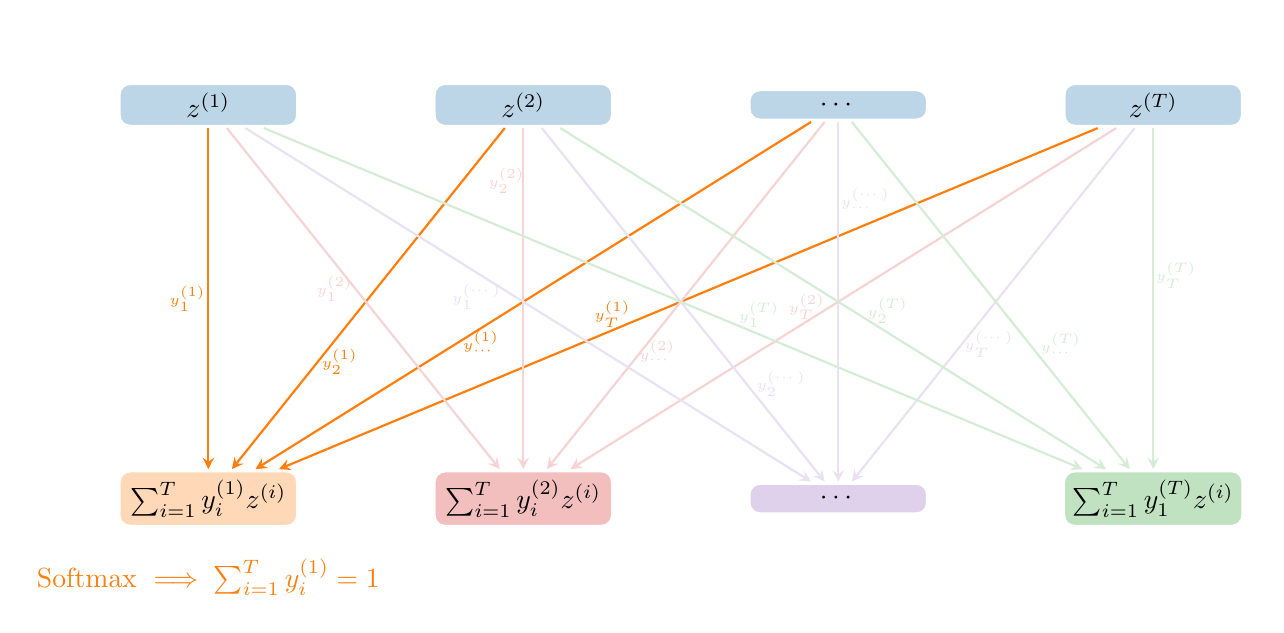
\begin{tikzpicture}[module/.style={draw, very thick, rounded corners, minimum width=15ex},
    output1/.style={module, fill=morange!30},
    output2/.style={module, fill=mred!30},
    output3/.style={module, fill=mpurple!30},
    output4/.style={module, fill=mgreen!30},
    input/.style={module, fill=mblue!30},
    arrow/.style={-stealth, thick, rounded corners},
    color=white,
]

    \node[output1] (o1) {\color{black}$\sum_{i=1}^Ty^{(1)}_iz^{(i)}$};
    \node[output2, left of=o1, xshift=5cm] (o2) {\color{black}$\sum_{i=1}^Ty^{(2)}_iz^{(i)}$};
    \node[output3, left of=o2, xshift=5cm] (output_dots) {\color{black}$\cdots$};
    \node[output4, left of=output_dots, xshift=5cm] (oT) {\color{black}$\sum_{i=1}^Ty^{(T)}_1z^{(i)}$};

    \node[input, above of=o1, yshift = 4cm] (z1) {\color{black}$z^{(1)}$};
    \node[input, above of=o2, yshift = 4cm] (z2) {\color{black}$z^{(2)}$};
    \node[input, above of=output_dots, yshift = 4cm] (input_dots) {\color{black}$\cdots$};
    \node[input, above of=oT, yshift = 4cm] (zT) {\color{black}$z^{(T)}$};

    \node[fit=(z1)(z2)(input_dots)(zT),draw, ultra thick, rounded corners, label=above:{$input$ sequence}] (input) {};
    \node[fit=(o1)(o2)(output_dots)(oT),draw, ultra thick, rounded corners, label=below:{$output$ sequence}] (output) {};

    \draw[arrow, color=morange] (z1) -- (o1) node[midway, left, xshift=.1cm] {\tiny$y^{(1)}_1$};
    \draw[arrow, color=morange] (z2) -- (o1) node[midway, left, yshift = -.8cm] {\tiny$y^{(1)}_2$};
    \draw[arrow, color=morange] (input_dots) -- (o1) node[midway, left, yshift = -.6cm, xshift = -.3cm] {\tiny$y^{(1)}_{\cdots}$};
    \draw[arrow, color=morange] (zT) -- (o1) node[midway, left, yshift = -.2cm, xshift = -.6cm] {\tiny$y^{(1)}_T$};

    \draw[arrow, color=mred!20] (z1) -- (o2) node[midway, above left, yshift = -.17cm] {\tiny$y^{(2)}_1$};
    \draw[arrow, color=mred!20] (z2) -- (o2) node[midway, above left, yshift = 1.2cm, xshift = .15cm] {\tiny$y^{(2)}_2$};
    \draw[arrow, color=mred!20] (input_dots) -- (o2) node[midway, above left, yshift = -1cm] {\tiny$y^{(2)}_{\cdots}$};
    \draw[arrow, color=mred!20] (zT) -- (o2) node[midway, above left, yshift=-.4cm, xshift=-.1cm] {\tiny$y^{(2)}_T$};

    \draw[arrow, color=mpurple!20] (z1) -- (output_dots) node[midway, right, xshift = -1.1cm, yshift=.1cm] {\tiny$y^{(\cdots)}_1$};
    \draw[arrow, color=mpurple!20] (z2) -- (output_dots) node[midway, right, yshift = -1cm, xshift=.8cm] {\tiny$y^{(\cdots)}_2$};
    \draw[arrow, color=mpurple!20] (input_dots) -- (output_dots) node[midway, right, yshift = 1.3cm, xshift = -.1cm] {\tiny$y^{(\cdots)}_{\cdots}$};
    \draw[arrow, color=mpurple!20] (zT) -- (output_dots) node[midway, right, yshift = -.5cm, xshift=-.5cm] {\tiny$y^{(\cdots)}_T$};

    \draw[arrow, color=mgreen!20] (z1) -- (oT) node[midway, above right, yshift = -.5cm, xshift = .7cm] {\tiny$y^{(T)}_1$};
    \draw[arrow, color=mgreen!20] (z2) -- (oT) node[midway, above right, yshift = -.45cm, xshift=.3cm] {\tiny$y^{(T)}_2$};
    \draw[arrow, color=mgreen!20] (input_dots) -- (oT) node[midway, above right, xshift = .5cm, yshift = -.9cm] {\tiny$y^{(T)}_{\cdots}$};
    \draw[arrow, color=mgreen!20] (zT) -- (oT) node[midway, above right, xshift=-.1cm] {\tiny$y^{(T)}_T$};

    \node[below of=o1, color = morange] (sum) {Softmax $\implies\sum_{i=1}^Ty^{(1)}_i = 1$};


\end{tikzpicture}
\end{document}